\cotefile{12}
\scanpage{2}
% archive foliation: 1 (upper right; also lower left)
\uline{Esquisse d'une théorie des motifs.}

1. Revue des théories cohomologiques habituelles des schémas projectifs lisses.
L'idée de motifs, \inserted{\unsure{qui doit remplacer|que doit remplir} la cohomologie \unsure{entière} (en terme des modules de \unsure{t.f.|déf.} sur $\mathbb{Z}$ !).}
\unsure{Réserves} : a) Isomotifs, b) Motifs $\frac12$ simples c) Base ponctuelle.
\margin{*}

2. Définition de la catégorie $\mathcal{M}^+(k)$ des motifs effectifs sur $k$.
C'est une catégorie abélienne \inserted{``$\frac12$ simple''} avec $\otimes$.
Foncteurs $T^{\unsure{*}}_{\mathrm{DR}}$, $T_{\mathrm{Hdg}}$ (si $k$ de car nulle), $T_B$ (si $k=\mathbb{C}$), $T^\ell$ (si $\ell\ne\deleted{\unsure{car}}\inserted{\operatorname{car}}k$) \deleted{\illegible{3}} ces foncteurs sont multiplicatifs. Tous ces foncteurs sont fidèles.

3. Graduation dans la catégorie $\mathcal{M}^+(k)$. Les foncteurs $h^i(X)$.\unsure{$\mathcal{M}^{+i}(k)$}.
\inserted{Le produit $\otimes$ compatible avec graduation.}

4. L'équivalence $\mathcal{M}^{+1}(k)^\circ\simeq\operatorname{Isab}(k)$
($X\mapsto\underline{\operatorname{Pic}}^0_X$, $A\mapsto h^1(\widehat A)$).

\deleted{4. Le motif $\mathbb{Q}(-1)$, et la catégorie $\mathcal{M}(k)$ des motifs \unsure{et}}
\margin{*}
Les motifs de poids $\geq1$ comme généralisation des VA. Le \unsure{caractère} ``discret'' est conservé (s'exprimant \unsure{alg.ment} par le fait que si $k\longrightarrow k'$ est une extension de corps algébriquement clos, alors $\mathcal{M}^{\unsure{e}}(k)\unsure{-|\longrightarrow}\mathcal{M}^{\unsure{e}}(k')$ est pleinement fidèle).

\unsure{Caractère} continu\dots\ Exemples d'énoncé suggéré par la théorie des \deleted{schémas} abéliens : caractérisation des motifs \uuline{lisses} sur $S$ \deleted{\unsure{géométriquement réduit}}\inserted{normal}\deleted{\unsure{et connexe}}.
\margin{*}

5. Le motif $\mathbb{Q}(\unsure{-1|+1})$ (anti-Tate). La catégorie $\mathcal{M}(k)$ des motifs (isomotifs semi-simples sur $k$ !). Maintenant il y a des \uline{Hom} internes, en plus des $\otimes$ et de la graduation.

Si $\mathcal C$ est une catégorie pseudo-abélienne avec $\otimes$, alors les foncteurs compatibles avec $\otimes$ de $\mathcal{M}(k)$ dans $\mathcal C$ correspondent aux foncteurs $T:V(k)^\circ\longrightarrow\mathcal C$, satisfaisant Künneth, et tels que \deleted{\unsure{$\mathbb{P}^1_k$}} $T(\mathbb{Q}(-1))=\operatorname{Im}T(\pi)$
($\pi$ le projecteur dans $h(\mathbb{P}^1_k)$ \deleted{\illegible{1}}, d'im.\ $h^2(\mathbb{P}^1_k)=\mathbb{Q}(-1)$)
\uline{soit inversible}. On montre qu'un tel $T$ commute automatiquement à la formation des \uline{Hom}. La catégorie des motifs $\mathcal{M}(k)$ est donc caractérisée, avec sa structure $\otimes$, \deleted{et l'objet $\mathbb{Q}(\unsure{-1})$} à équivalence près par propriété universelle.

\scanpage{3}
% archive foliation: 2 (upper right and lower left)
6. \uline{Niveau d'un motif}

\inserted{Résulte de la \unsure{présence} de $\mathcal{M}^+$ dans $\mathcal{M}$.}
Un motif $M$ est dit \uline{de niveau} $\leq i$ s'il est de la forme $M'(n)$, où $M'\in\operatorname{Ob}\mathcal{M}^+(k)$ est à composantes homogènes de degrés $\leq i$. On dit que $M$ est purement de niveau $i$ s'il est de niveau $\leq i$, et si aucun sous-motif $\ne0$ n'est de niveau $\leq i-1$.
\inserted{Cet $i$ est unique et $\geq0$.}
Tout motif \inserted{$M$} se décompose \inserted{de façon unique} en somme de motifs purs de niveau $i$
\[
M=\coprod_{i\in \mathbb{Z}}M_i
\]
donc s'il est de \deleted{degré} poids $n$, \deleted{il s'écrit}
\inserted{(les $i$ tels que \uuline{$M_i$}$\ne0$ ont la parité que $n$, et}
\[
M=\coprod_iM'_i\left(\frac{\unsure{n-i|i-n}}2\right)
\qquad M'_i\in\text{\figure{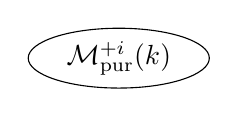
\begin{tikzpicture}[baseline=(m.base)]
\node (m) at (0,0) {$\mathcal{M}^{+i}_{\mathrm{pur}}(k)$};
\draw (0,0) ellipse (1.15 and .38);
\end{tikzpicture}}}
\]
où $M'_i$ est \deleted{\unsure{purement de poids}}\inserted{\uline{effectif}} pur de poids et niveau $i$.

\margin{\unsure{Exemp.} : si $i>n=\dim X$, alors $h^i(X)$ est \uline{de niveau} $\leq2n-i<i$.}

\deleted{\unsure{Ceci signifie}} Les motifs de \deleted{poids}\inserted{niveau} $\leq i$ sont ceux qui, modulo twist de Tate, ``proviennent'' des variétés $X\in V(k)$ de dimension $\leq i$. Ceci résulte du fait que $h(X)$ est de niveau $\leq\dim X$, et que \deleted{\unsure{d'ailleurs}} si $i\leq\dim X$, $h^i(X)\hookrightarrow h^i(Y)$, où $Y$ est une section linéaire de dim $i$ (au sens du ``th. de Lefschetz''). Autre interprétation en termes de cohomologie $\ell$-adique
\deleted{(en supposant $k$ alg. clos, ce qui est loisible, car la notion de niveau, \unsure{pureté de niveau}, est invariante par extension du corps de base)}
On regarde dans $H^i(\overline X,\mathbb{Q}_\ell)$ la ``filtration géométrique'' définie par
\[
\operatorname{Filt}^{j}H^i(X,\mathbb{Q}_\ell)
=\underset{U,\ U\text{ ouvert \unsure{tels que}}\ \operatorname{codim}(X-U)\geq j}{\unsure{\varinjlim|\lim}}
\operatorname{Ker}\bigl(H^i(X,\mathbb{Q}_\ell)\longrightarrow H^i(U,\mathbb{Q}_\ell)\bigr)
\]
\margin{\uline{Ex} Si $i\geq n=\dim X$\quad $h^i(X)$ est de niveau $\leq2n-i$.}

\scanpage{4}
% archive foliation: 3 (upper right and lower left)
Alors on a, \deleted{si $X$ purement de dim $n$ et $i\leq n$ (resp.\ $i\geq n$)}
\[
\begin{aligned}
\operatorname{Filt}^{j}H^i(\overline X,\mathbb{Q}_\ell)
={}&\text{partie de }T^\ell(h^i(X))\ \deleted{\text{provenant}}\inserted{\text{image}}\text{ du}\\
&\text{plus grand sous-motif de}\\
&\text{niveau }\leq i-2j\quad
\deleted{(\text{resp. }\unsure{2n-i-2j|2n-i-j})}\ 
\deleted{\text{de}}\inserted{\text{de}}\ h^i(X)
\end{aligned}
\]

Cette caractérisation \inserted{du niveau des motifs} est \unsure{tout} au moins correcte si on admet la résolution des singularités, \deleted{sur $k$}\inserted{des variétés de dim $\leq\dim X=n$ sur $k$.}
Comme conséquence de la résolution et des conjectures \unsure{standards|standarts}, on trouve donc que les dimensions des $\operatorname{Filt}^jH^i(\overline X,\mathbb{Q}_\ell)$ sont indépendantes de $\ell$.
(Bien mieux, ils correspondent à des motifs, et les \unsure{petits} facteurs successifs sont \deleted{\unsure{et}} purs de poids $i-2j$ resp $\unsure{2n-i-j|2n-i-2j}$).
\margin{Parler des inv. birationnels\dots}
\margin{Conjectures de Tate et de Hodge pourraient \uuline{passer ici}.}

7. \uline{Structure des $\otimes$-catégories}. \deleted{\unsure{abéliennes}}

\deleted{\unsure{Catégorie}} Catégorie abélienne avec opération $\otimes$ ``ass.'', ``comm.'' et ``unitaire''. On suppose de plus l'existence de \uline{Hom} internes, au sens de $\otimes$.
On dit qu'elle est ``rigide'' si
\[
\check M\otimes N\xrightarrow{\sim}\underline{\operatorname{Hom}}(M,N)
\]
Supposons de plus que $\mathcal C$ soit $K$-linéaire ($K$ un corps)
(\unsure{revient} à donner $K\longrightarrow\operatorname{End}(\operatorname{id}_{\mathcal C})$), et que les Hom soient de dim finie sur $k$ : \deleted{\unsure{ce est}} On dira qu'on a une $\otimes$-catégorie sur $k$ (pour simplifier).
Une telle catégorie est dite ``connexe'' si
\[
\operatorname{End}(\mathbf1_{\mathcal C})\simeq K\qquad(\unsure{par}\text{ l'identité}).
\]

\scanpage{5}
% archive foliation: 4 (upper right and lower left)
Exemple : Si $G$ est un groupe algébrique sur $K$, la catégorie $\operatorname{Modf}(G)$ des vectoriels sur lesquels $\unsure{K|G}$ opère. Idem avec groupes proalgébriques (p.ex.\ profinis).
Cet exemple est essentiellement universel, comme on va voir.

$\otimes$-foncteurs. Foncteurs fibres \inserted{sur $K$, -- sur $K'$, \dots}.
Considérons un couple $(\mathcal C,F)$ \deleted{\unsure{cf}} d'une $\otimes$-catégorie sur $K$, avec foncteur fibre rat.\ $/K$. À cette situation on peut associer un groupe \deleted{\unsure{aff}}\inserted{$G$} affine sur $K$ (ou pro-groupe \unsure{pro-affine} sur $K$), et une équivalence
\[
(\mathcal C,F)\simeq(\operatorname{Modf}(G),\text{oubli}).
\]
\margin{$G(A)=\operatorname{Aut}F_A$\quad
$F_A\inserted{(M):=F(M)\unsure{\otimes_K|\otimes}A}$ \deleted{\unsure{considéré}}
comme foncteur fibre à valeurs dans $\operatorname{Mod}(A)$.}

De façon précise, associant à chaque $G$ le couple $\unsure{((\operatorname{Modf}),G),\mathrm{oubli})|(\operatorname{Modf}(G),\mathrm{oubli})}$, on trouve un foncteur
\diagram{\begin{tikzcd}[column sep=large]
\text{groupes affines sur }K \arrow[r] &
\begin{gathered}
\otimes\text{-catégories avec foncteur}\\
\text{fibre donné, avec }\otimes\\
\text{-foncteurs mod isom,}\\
\text{compatibles avec }F
\end{gathered}
\end{tikzcd}}
et ce foncteur est pleinement fidèle.

\[
\mathcal C\text{ ``de type fini''}\Longleftrightarrow G\text{ de type fini}
\]
\[
\mathcal C\text{ $\frac12$-simple}
\underset{\inserted{\text{si }K\text{ de car. nulle}}}{\Longleftrightarrow}
\deleted{G\text{ \unsure{réductif}}}\quad G\text{ (pro)réductif}.
\]
\deleted{\unsure{G proalgébrique}}

\uline{Pb} Possibilité d'une définition des autres op.\ tensorielles telles $\wedge$, $\operatorname{Sym}^i$ (en fait, on voit que c'est indépendant de l'existence et du choix de $\unsure{\varphi|F}$).

Si on a un foncteur fibre, tout autre foncteur fibre $F'$ s'obtient en ``tordant'' avec un protorseur $P$ sous $G$, $P=(\unsure{P_i|B_i})$ :
\[
F'=P\times^G F
\]
\margin{\uuline{à prouver}}
\margin{\unsure{Réserves} : Affirmer que si $\mathcal C$ de type fini, deux foncteurs fibres deviennent isom.\ sur ext.\ finie.}

\scanpage{6}
% archive foliation: 5 (upper right and lower left)
Alors
\[
G'=P\times^G G=\operatorname{ad}(P)
\]
En fait, il y a des cas intéressants où \deleted{\unsure{ne|on}} on peut trouver aucun foncteur fibre. Mais si $\mathcal C$ est de type fini, alors on \inserted{doit pouvoir} montrer qu'on peut trouver un foncteur fibre sur une extension finie de $K$.
\deleted{On \unsure{réussit} ainsi à décrire les}
\inserted{Quand il en est ainsi, \deleted{on doit \unsure{arriver}},}
admettant le résultat ``d'unicité'' de foncteurs fibres, \deleted{on doit} arrive à décrire $(\mathcal C,F)$ intrinsèquement en termes d'une gerbe sur un site convenable\dots

8. \uline{\unsure{Cas des catégories|Cas de catégorie} des motifs.}
\deleted{\uuline{lien avec le groupe fondamental profini.}}

$S$ schéma régulier. \inserted{connexe}
On définit $\mathcal{M}^+(S)$, $\mathcal{M}(S)$ en paraphrasant ce qui est fait sur un corps, en travaillant \unsure{les|avec} $X$ projectif lisse sur $S$, avec $C(X)\overset{\mathrm{def}}=C(X_\eta)$ ($\eta$ pt générique de $S$).
Ainsi, $\mathcal{M}(S)\unsure{-|\longrightarrow}\mathcal{M}(\eta)$ est pleinement fidèle, permettant d'interpréter $\mathcal{M}(S)$ comme ss-catégorie pleine de $\mathcal{M}(\eta)$.
De plus, pour $\forall$ morphisme $f:S'\longrightarrow S$ de schémas réguliers, on définit $f^*:\mathcal{M}(S)\longrightarrow \mathcal{M}(S')$ un $\otimes$-foncteur correspondant (c'est ici que sert l'hypothèse de \uline{régularité} sur les schémas\dots).
\margin{à expliciter\dots}

Tout point \inserted{géom.} \uline{complexe} de $S$ définit un foncteur fibre ``de Betti'' \deleted{$\unsure{F_{\mathrm{Betti}}=F_\xi}$}
\[
F_{\unsure{\xi|\zeta}}^{\mathrm{Betti}}=F_{\unsure{\xi|\zeta}}^B:
\mathcal{M}(S)\unsure{-|\longrightarrow}\operatorname{Modf}(\mathbb{Q}),
\]
d'où un groupe proalgébrique $G$ sur $\mathbb{Q}$, pro-réductif

\scanpage{7}
% archive foliation: 6 (upper right and lower left)
en fait, \deleted{et} décrivant $\mathcal{M}(S)$.
Pratiquement, on n'a guère qu'à considérer dans \deleted{\unsure{une}} chaque question une ss-catégorie de type fini de $\mathcal{M}(S)$, soit $\mathcal C$. Elle est alors décrite par un \deleted{\unsure{proalgébrique}} groupe algébrique \inserted{réductif} $G$ sur $\mathbb{Q}$.
Question intéressante : comment sont reliés ces groupes pour des $\unsure{\xi|\zeta}$ différents (ils se déduisent tous les uns des autres par torsion\dots).
Déjà intéressant si $S$ est le spectre d'une ext.\ finie $k$ de $\mathbb{Q}$\dots!

Si $S$ est de car.\ $p>0$, on ne pourra en général trouver de foncteur fibre sur $\mathbb{Q}$ (contre-exemple de Serre, lié aux courbes elliptiques de Hasse nul).
Mais on aura un foncteur fibre sur $\mathbb{Q}_\ell$ pour $\forall$ pt géom de car.\ $\ne\ell$, d'où un foncteur fibre sur une extension finie \inserted{$K/$} de $\mathbb{Q}$ (si on se restreint à une $\mathcal C\subset \mathcal{M}(S)$, stable par \deleted{$\unsure{\otimes,\check{\phantom M}}$} $\otimes,\vee$, et à \unsure{engendrement} fini\dots).
Donc on trouve un groupe algébrique réductif $G_K$ sur $K$, qui permet de représenter la catégorie des $K'$-motifs pour $\forall$ corps de \unsure{coeff} $K'$ qui est une extension de $K$.

\margin{Structure $\varepsilon,\unsure{D}$, \unsure{graduations} $\unsure{\gamma_1},\unsure{\gamma_2}$
\inserted{$\unsure{\exp(D)=\lambda}$}
\deleted{\unsure{prolongement de} \illegible{2} $\unsure{C}$ \illegible{1}}
$\unsure{T}^{\unsure{*}}_{\mathrm{Hdg}}$.}
9) \uline{Relations avec le $\pi_1$, \unsure{profini}} :
\inserted{(A) $\unsure{G/G^0}\unsure{-|\longrightarrow}\unsure{\pi^1|\pi_1}$.}
Soit $F$ un foncteur fibre à coefficients dans $K$ sur $\unsure{\mathcal{M}(C)|\mathcal{M}(S)}$,
$\unsure{\xi|\zeta}$ un pt géométrique. On dit que $F$ et $\unsure{\xi|\zeta}$ sont associés si on a un \unsure{isom}

\scanpage{8}
% archive foliation: 7 (upper right and lower left)
\[
F|\mathcal{M}^{+0}(S)\simeq F_{\unsure{\xi|\zeta}}
\]
où $F_{\unsure{\xi|\zeta}}$ est le foncteur évident sur $\mathcal{M}^{+0}(S)$ : fibre en $\unsure{\xi|\zeta}$.
(NB. $S$ étant connexe, ces foncteurs sont isom entre eux, donc la \uline{condition} d'association ne dépend pas de $\unsure{\xi|\zeta}$. Mais il faut le considérer plutôt comme une \uline{donnée} supplémentaire, comme \uline{donnée} de l'isom en question).

\uline{Ex 1} Si source $\unsure{\xi|\zeta}=\operatorname{Spec}(\mathbb{C})$, \deleted{alors} $F=F_{\unsure{\xi|\zeta}}^{\mathrm{Betti}}$, alors on a une telle donnée.
\inserted{\uline{Ex. 2}\quad $T^\ell_{\unsure{\xi|\zeta}}$.}

\uline{Ex 3} Si $S=\operatorname{Spec}k$, $k$ corps de car.\ nulle (p.ex.\ $k=\mathbb{Q}$) et si $F$ est le foncteur fibre \deleted{sur}\inserted{à coefficients dans} $k$ $T_{\mathrm{DR}}$, \deleted{alors} ou $T_{\mathrm{Hdg}}$, alors il n'est pas en général associé aux pts géométriques.

\uline{Ex 4} Si \deleted{$k$ est} $S$ est le spectre d'un corps alg clos, alors $\forall$ $F$ est associé à $\unsure{\xi|\zeta}$, du moins si $k$ est dénombrable, \inserted{i.e.\ de degré de transc.\ absolu dénombrable}, donc $\mathcal{M}(k)$ à engendrement dénombrable\dots

\deleted{Alors on trouve un isom canonique
\[
\left\{\begin{aligned}
\pi_1(S,\unsure{\xi|\zeta})&\simeq\varprojlim G_\alpha/G_\alpha^0\\
\text{les }G_\alpha/G_\alpha^0&\text{ sont des groupes constants}\\
&\text{sur }K\ \dots
\end{aligned}\right.
\]
\unsure{Cela|Ceci} résulte du \deleted{fait que} $\otimes$-foncteur canonique
\diagram{\begin{tikzcd}
\operatorname{Mod}\,\unsure{\mathrm{fin}|\mathrm{cont}}(\pi_1)\simeq \mathcal{M}^{+0}(S)
\arrow[r] & \mathcal{M}(S)
\end{tikzcd}}
qui définit
\diagram{\begin{tikzcd}
G\arrow[r]&\pi_1
\end{tikzcd}}
}

\scanpage{9}
% Pencil foliation: 8, upper right and lower left.
Alors on trouve un $\otimes$-foncteur \inserted{pleinement} fidèle
\diagram{\begin{array}{c}
\pi_1\text{-}\mathbb{Q}\text{-modules admissibles de rang fini sur }\mathbb{Q}\\
\longrightarrow\quad\text{motifs sur }S
\end{array}}
qui est décrit par un \inserted{épi}morphisme
\diagram{\begin{tikzcd}
G=\varprojlim G_\alpha \arrow[r] & \pi_1(S,\unsure{\xi|\zeta})
\end{tikzcd}}
et se factorise donc en un \uline{épimorphisme} canonique
\margin{$*$}
\diagram{\begin{array}{|ccc|}\hline
\varprojlim_\alpha G_\alpha/G_\alpha^0&\longrightarrow&\pi_1(S,\unsure{\xi|\zeta})\\\hline
\end{array}}
Soit $\pi'_1$ le premier mb. Alors \deleted{les}
\inserted{(supposant $K=\mathbb{Q}$} \deleted{$\pi'_1$}
pour simplifier) les $\pi'_1$-$\mathbb{Q}$-modules
correspondent à la sous-catégorie de $\mathcal{M}(S)$ formée
des motifs \inserted{$M$} tels que la sous-\inserted{$\otimes$-}catégorie engendrée
par $M$ soit de ``longueur finie''. Utilisant
conjecture de Tate (ou de Hodge si $S$ de
car. générique nulle) on \inserted{peut} voi\deleted{t}\inserted{\unsure{r}} que ce sont les
motifs de \deleted{\unsure{poids}} niveau \inserted{et poids} zéro, \inserted{i.e. les motifs effectifs de poids zéro,}
i.e. que \uline{c'est un
isomorphisme}. Les \deleted{résultats}\inserted{réflexions} précédentes peuvent
se \deleted{\unsure{faire}}\inserted{développer} aussi (utilisant la notion de
motif sur $S$ à coeff. dans $K$) si on ne suppose
pas $K=\mathbb{Q}$.

\deleted{\unsure{NB} \illegible{2} \unsure{objets} de \unsure{$\alpha$} \unsure{que}}

\uline{NB} Soit $S'\longrightarrow S$ un morphisme
étale \inserted{\unsure{surj.}}\deleted{de} $S$, \inserted{d'avance,} et supposons que $F$ provienne d'

% Printed letterhead, upside down relative to the handwriting, lower right.
INSTITUT

DES HAUTES ETUDES SCIENTIFIQUES

91 - BURES-SUR-YVETTE

928 48-53

\scanpage{10}
% Pencil foliation: 9, upper right and lower left.
un \deleted{\unsure{certain}} $\otimes$-foncteur \deleted{$F'$} sur $S'$. Alors,
comme en théorie du groupe fondamental ordinaire,
$G'\longrightarrow G$ est un monomorphisme, dont
l'image est le \deleted{\unsure{groupe}} l'image inverse \inserted{dans $G$} du sous
groupe ouvert de $\pi_1(S,\unsure{\xi|\zeta})$ qui correspond à $S'/S$.
On en conclut que la bijectivité de \unsure{$(*)$}
\deleted{équivaut \unsure{lorsque} \illegible{2} $S=$ \unsure{1}}
(pour tout $S$, disons) équivaut au fait que
pour $S=\operatorname{Spec}k$, $k$ alg. clos, le \deleted{\unsure{le}} groupe $G$
est \uline{connexe}.

10) \uline{Relations avec le $\pi_1$ profini : les homs $\pi_1\longrightarrow G(\mathbb{Q}_\ell)$.}

Supposons \deleted{\unsure{encore}} que $K\hookrightarrow\mathbb{Q}_\ell$ ;
\deleted{et que}\inserted{on dit que} $F$
\deleted{est associé au pt géom. $\unsure{\xi|\zeta}$}.
\uline{compatible avec
le foncteur de Tate} $\inserted{T^\ell_{\unsure{\xi|\zeta}}}$
(pour le plongement donné
de $K$ dans $\mathbb{Q}_\ell$) si
\[
 F\otimes_K\mathbb{Q}_\ell \xrightarrow{\sim}T^\ell_{\unsure{\xi|\zeta}}
\]
(donnée de compatibilité avec foncteur de
Tate). \uline{Exemple} 1 \quad $K=\mathbb{Q}_\ell,\ F=T^\ell_{\unsure{\xi|\zeta}}$,

\uline{Exemple} 2 \quad $K=\mathbb{Q},\ F=T^{\unsure{\xi|\zeta}}_{\mathrm{Betti}}$,
$\unsure{\xi|\zeta}$ un pt complexe

Alors \deleted{\unsure{ceci}} l'homomorphisme canonique
\diagram{\begin{tikzcd}
\pi_1(S,\unsure{\xi|\zeta}) \arrow[r] & \operatorname{Aut}T^\ell_{\unsure{\xi|\zeta}}
\end{tikzcd}}
\deleted{définit un}
puis :
\[
\operatorname{Aut}T^\ell_{\unsure{\xi|\zeta}}
 \simeq \operatorname{Aut}F\otimes_{\unsure{K}}\mathbb{Q}_\ell
 \simeq G(\mathbb{Q}_\ell).
\]
définit un homomorphisme
\diagram{\begin{array}{|ccc|}\hline
\varphi_\ell:\pi_1(S,\unsure{\xi|\zeta})&\longrightarrow&G(\mathbb{Q}_\ell)\\\hline
\end{array}}

\scanpage{11}
% Pencil foliation: 10, lower left.
INSTITUT

DES HAUTES ETUDES SCIENTIFIQUES

91 - BURES-SUR-YVETTE

928 48-53

\scanpage{12}
% Pencil foliation: 10, upper right; 11, lower left.
Noter que si $F$ est compatible avec $T^\ell_{\unsure{\xi|\zeta}}$, il est
à fortiori \uline{associé à} $\unsure{\xi|\zeta}$, et on trouve
\diagram{\begin{tikzcd}
G\deleted{\unsure{\mathbb{Q}}}\arrow[r]&\pi_1(S,\unsure{\xi|\zeta})
\end{tikzcd}}
d'où
\diagram{\begin{tikzcd}
\unsure{\psi_\ell|\eta_\ell}:G(\mathbb{Q}_\ell)\arrow[r]&\pi_1(S,\unsure{\xi|\zeta})
\end{tikzcd}}
On voit tout de suite que cet homomorphisme
est inverse à gauche de $\varphi_\ell$
\[
 \boxed{\unsure{\psi_\ell|\eta_\ell}\varphi_\ell
   =\operatorname{id}_{\pi_1(S,\unsure{\xi|\zeta})}}
\]
Si on s'intéresse à une sous-catégorie $C_\alpha$ de $C$,
correspondant à un $\unsure{G_\alpha^0|G_\alpha}$, alors $G_\alpha/G_\alpha^0$
\deleted{\unsure{correspond}}\inserted{définit}
\deleted{\unsure{quotient}} un quotient $\pi_\alpha$ de $\pi_1(S,\unsure{\xi|\zeta})$,
et on a
\diagram{\begin{tikzcd}
& G_\alpha/G_\alpha^0 \arrow[dr,dashed] &\\
\pi_1(S,\unsure{\xi|\zeta})\arrow[r,"\varphi_\ell"]
 \arrow[rr,bend right=32,swap,"\uline{\text{hom can.}}"]
 & G_\alpha(\mathbb{Q}_\ell)\arrow[ur,dashed]\arrow[r]&\pi_\alpha
\end{tikzcd}}
(commutatif).

La conjecture de Tate \inserted{(avec action semi-simple de Galois !)}
équivaut à dire que, si
$S$ est localisé d'un schéma de type fini sur $\mathbb{Z}$, alors
$G_\alpha\unsure{\otimes|\times}_{\mathbb{Q}_\ell}$ est
l'enveloppe algébrique de $\operatorname{Im}(\pi_1(\uline{S,\unsure{\xi|\zeta}})
\longrightarrow G_\alpha(\mathbb{Q}_\ell))$.

\margin{\uline{NB} La conjecture
de Tate sous la
forme : les \unsure{$\frac12$-invariants}
dans $H^{2i}(\overline X,\mathbb{Q}_\ell(i))$
sont les comb.
à coeff. dans $\mathbb{Q}_\ell$
des classes algébriques
--- implique (avec
conjectures standard)
la $\frac12$ simplicité dans
Tate ---}

\margin{\deleted{\fbox{\begin{tabular}{l}
\unsure{l'image} \illegible{4}\\
\unsure{$\pi_1$} \illegible{2} \unsure{$(M)$}\\
\illegible{4}
\end{tabular}}}}

11) \uline{Cas} $S=\operatorname{Spec}k$, $k$ \uline{corps fini}.

$C\subset \mathcal{M}(k)$, et $F$ un ``foncteur'' fibre sur
$C$ à coeff dans $K$. Comme on a un élément
canonique de
\diagram{\begin{tikzcd}
\operatorname{Frob}_k\in\operatorname{Aut}\underline{\operatorname{Id}}_{\mathcal{M}(k)}
 \arrow[r]&\operatorname{Aut}\operatorname{id}_C
 \left[\simeq\unsure{Z|\mathfrak Z}(\mathbb{Q})\right]
\end{tikzcd}}
\margin{\inserted{\unsure{$Z$} est le centre de $G$}\deleted{\unsure{$Z(K)$}}}
on en déduit un élément canonique de
$G(K)=\operatorname{Aut}F$, et même de $\unsure{Z|\mathfrak Z}(\mathbb{Q})$
($\unsure{Z|\mathfrak Z}$ est le centre de $G$)
\[
 \boxed{\operatorname{Frob}_{k,F}\in
 \unsure{Z|\mathfrak Z}(\mathbb{Q})\subset G(K)}.
\]
\margin{\fbox{\begin{tabular}{l}
NB. $\unsure{Z|\mathfrak Z}$ est\\
en fait défini\\
sur $\mathbb{Q}$ !
\end{tabular}}}

\scanpage{13}
% Pencil foliation: 11, upper right; 12, lower left.
Si $K\subset\mathbb{Q}_\ell$ et si $F$ est compatible avec
$T^\ell_{\unsure{\xi|\zeta}}$, alors l'image de
$\operatorname{Frob}_{k,F}\in\unsure{Z|\mathfrak Z}(K)
\unsure{=|\subset}\unsure{Z|\mathfrak Z}(\mathbb{Q}_\ell)\subset G(\mathbb{Q}_\ell)$
\deleted{n'est autre}
\deleted{\unsure{par l'hom}}
n'est autre que l'image du
générateur
\[
 \operatorname{Frob}_k\in\pi_1(k,\unsure{\xi|\zeta})\simeq\widehat{\mathbb{Z}}
\]
par l'hom
\diagram{\begin{tikzcd}
\varphi_\ell:\widehat{\mathbb{Z}}\arrow[r]&G(\mathbb{Q}_\ell)
\end{tikzcd}}

La \uline{conjecture de Tate} pour le corps
fini $k$ équivaut à dire que $G$ est
l'enveloppe algébrique du \unsure{ss-groupe|sous-groupe} engendré
par $\operatorname{Frob}_{k,F}\in G(K)$.
Elle implique donc
que $G$ est commutatif. [Comme il est
défini mod twist, on voit qu'il est en
\unsure{fait can.} défini sur $\mathbb{Q}$, canoniquement, et
évidemment on aura en fait, alors
\[
 \operatorname{Frob}_{k,F}\in\deleted{\unsure{Z|\mathfrak Z}(\mathbb{Q})\subset}G(\mathbb{Q})
\]
].

\uline{Conséquence de conjecture de Tate pour $k$.}

$G$ est extension \deleted{(\unsure{commutative et torique})}
de $\widehat{\mathbb{Z}}$ par un tore resp. protore.

\uline{Conséquence} : Soit à nouveau $S$ quelconque,
mais muni d'un point fermé $s$ tel que
$k(s)=k$ soit fini. Soit $C\subset \mathcal{M}(S)$,
\deleted{\unsure{et soit}}\inserted{muni}
\deleted{$C$ une sous-catégorie de}
d'un foncteur fibre $F$,
à coeff. dans un corps $K\supset\mathbb{Q}$,

\scanpage{14}
% Pencil foliation: 12, upper right; 13, lower left.
d'où un $G$ schéma en groupes sur $K$. Soit
$I_G$ le ``schéma des invariants'', isomorphe si $G$ connexe
à $T/W$ ($T$ tore maximal de $G$, $W$ le groupe de Weyl).
Alors on trouve un élément $f_s$ de $I_G(\mathbb{Q})$.
(NB. $I_G$ est en fait défini sur $\mathbb{Q}$).
On trouve
ainsi une famille d'éléments $(f_s)_{s\in S^0}$, où $S^0$
désigne l'ens des pts de $S$ tels que $k(s)$ soit
fini : famille des frobenius. Compatibilité avec
les homs
\diagram{\begin{tikzcd}
G\deleted{\unsure{(K)}}\arrow[r]&\pi_1(S,\unsure{\xi|\zeta})
\end{tikzcd}}
et les homs
\diagram{\begin{tikzcd}
\pi_1(S,\unsure{\xi|\zeta})\arrow[r]&G(\mathbb{Q}_\ell).
\end{tikzcd}}

\scanpage{15}
% Pencil foliation: 13, upper right; 14, lower left.
12) Structures supplémentaires sur le groupe de Galois
motivique : \inserted{structures associées aux}
graduations, filtrations, au motif de Tate.

On choisit une sous-\inserted{$\otimes$-}catégorie graduée
\deleted{la catégorie}
$C$ de $\mathcal{M}(S)$, avec un foncteur fibre $F$,
d'où groupe de Galois motivique $G$
\inserted{(à coeff dans $K$)}.

a) Une graduation de type $\Pi$ du foncteur fibre,
compatible avec $\otimes$, est équivalente à la donnée
d'un hom
\diagram{\begin{tikzcd}
T=D_K(\unsure{\Pi|\pi})\arrow[r]&G
\end{tikzcd}}
La graduation provient d'une graduation fonctorielle
de $M\inserted{\in C}$ lui-même ssi l'hom $T\longrightarrow G$ est
central. Par suite :

1°) La graduation \inserted{canonique} de type $\mathbb{Z}$ des objets de
$C$ définit un hom canonique
\diagram{\begin{tikzcd}
\unsure{\gamma|g}:\mathbb{G}_{\mathrm m,K}\arrow[r]&G
\end{tikzcd}}

2°) Si $F=T_{\mathrm{Hdg}}$, la bigraduation de ce
foncteur correspond à un hom
\deleted{\diagram{\begin{tikzcd}
D_K(\mathbb{Z}^2)=\mathbb{G}_{\mathrm m}^2\arrow[r]&G
\end{tikzcd}}
donc à deux \unsure{h}}
\diagram{\begin{tikzcd}
i:\mathbb{G}_{\mathrm m,K}^2\arrow[r]&G
\end{tikzcd}}
donc à deux hom commutant l'un à
l'autre
\diagram{\begin{tikzcd}
i_1,i_2:\mathbb{G}_{\mathrm m}\arrow[r]&G
\end{tikzcd}}
Comme la graduation totale associée est celle
de 1°), on trouve
\[
 i_1(\lambda)i_2(\lambda)=\unsure{\gamma|g}(\lambda)
\]
(ce qui entraîne déjà que $i_1,i_2$ commutent \dots).

\scanpage{16}
% Pencil foliation: 14, upper right; 15, lower left.
3°) Supposons $S=\operatorname{Spec}(\mathbb{C})$, prenons
$F=T_{\mathrm{Betti}}$\deleted{et $T_{\mathrm{Hdg}}$}.
\margin{\deleted{\unsure{bigr. de Hdg}}}
Alors on \deleted{peut prendre} $K=\mathbb{Q}$. D'autre part
$F\otimes_{\mathbb{Q}}\mathbb{C}\simeq T_{\mathrm{Hdg}}$
\deleted{\unsure{$\otimes_{\mathbb{Q}}\mathbb{C}$}},
donc
$G^{\mathrm{Betti}}\otimes_{\mathbb{Q}}\mathbb{C}\simeq G^{\mathrm{Hdg}}$
\deleted{\unsure{$\otimes_{\mathbb{Q}}\mathbb{C}$}}.
Donc dans $G^{\mathrm{Betti}}\otimes_{\mathbb{Q}}\mathbb{C}$ on trouve
\deleted{\unsure{$i$}} $i_1,i_2$
\diagram{\begin{tikzcd}
i_1,i_2:\mathbb{G}_{\mathrm m}\arrow[r]&G^{\mathrm{Betti}}\otimes_{\mathbb{Q}}\mathbb{C}
\end{tikzcd}}
tels que
\[
 i_1(\lambda)i_2(\lambda)=\unsure{\gamma|g}(\lambda).
\]
De plus on a
\[
 \overline{i_1(\lambda)}=i_2(\unsure{\lambda|\overline\lambda})
\]
ce qui exprime que les deux graduations
de Hodge sont conjuguées complexes l'une de
l'autre.

b) Il y a lieu de supposer que
$\operatorname{Ob}C\unsure{\ni|\supset}\mathbb{Q}(\unsure{-1|1})$.
Alors $\mathbb{Q}(\unsure{-1|1})$ \deleted{\unsure{est}} définit
un $G$-module $F(\mathbb{Q}(\unsure{-1|1}))$ de rang $1$,
d'où un hom
\diagram{\begin{tikzcd}
\varepsilon:G\arrow[r]&\mathbb{G}_{\mathrm m,K}
\end{tikzcd}}
Comme $\mathbb{Q}(-1)$ est de \deleted{\unsure{degré}} poids $2$, on aura
\[
 \boxed{\varepsilon(\unsure{\gamma|g}(\lambda))=\lambda^2}
\]

c) Supposons que sur le foncteur $F$ il y ait
une filtration fonctorielle, compatible avec \unsure{gr.}.
Comment l'exprimer ? On considère
\[
 F'=\operatorname{Gr}(F),
\]

\scanpage{17}
% Pencil foliation: 15, upper right; 16, lower left.
c'est un autre foncteur fibre, mais \uline{gradué},
donc défini par un \uline{torseur} $P\deleted{\unsure{G}}$ sur $G$, et
\inserted{$F$ se \unsure{trouve|déduit} de $F'$ par torseur $P'$ sur $G'$.}
Supposons que sur \deleted{\unsure{quelque part}} une extension
$K'$ de $K$, on puisse trouver un isom
$F\sim F'$ compatible avec les filtrations, et
induisant l'identité sur les gradués associés.
[\uuline{Ex} \inserted{$S=\operatorname{Spec}k$,} $k$ de car. nulle,
$F=T_{\mathrm{DR}}$ avec filtration
canonique ; ça marche encore si $S$ est n'importe
quel schéma \inserted{régulier} de car. nulle \dots].
Alors
il y a un sous-torseur \inserted{canonique} $Q$ de $P\deleted{\unsure{G}}$, de
groupe $H$ le sous-groupe de $G$ des autom
compatibles avec filtration et induisant l'identité
sur le gradué, et de \unsure{$=$|$\overline{\mathrm m}$} \deleted{\unsure{pour}} un $Q'$ dans
$P'$, \inserted{groupe $H'$.}
On notera que $H,H'$ sont unipotents. Ainsi,
$F$ se déduit canoniquement du foncteur
gradué $F'$ [\unsure{opération|application} définie par
\diagram{\begin{tikzcd}
\mathbb{G}_{\mathrm m,K}\arrow[r,"\alpha"]&G'
\end{tikzcd}}]
à l'aide d'un torseur $Q'$ sur le groupe
\inserted{unipotent} $H(\alpha)$ de $G'$ défini par $\alpha$ comme on verra.

\margin{\figure{\begin{tikzpicture}
\node[draw,ellipse,align=left] {expliciter\\la construc-\\tion de\\$H(\alpha)$};
\end{tikzpicture}}}

13) \uline{Relations avec le groupe de
\deleted{Galois}\inserted{Mumford-Tate}.}

\inserted{Les structures de Hodge polarisables forment une $\otimes$-catégorie
semi-simple. Tte sous-catégorie de type fini est ``définie'' par un
groupe alg. $G$ sur $\mathbb{Q}$.}

Soit $(V,V_0,(V^{p,q}))$ une structure de Hodge. $^{b}$

\margin{$b$ avec
$i_1,i_2:\mathbb{G}_{\mathrm m,\mathbb{C}}\longrightarrow G_{\mathbb{C}}$
satisfaisant $i_1(\lambda)i_2(\lambda)=i(\lambda)$ central,
$i_2(\lambda)=\overline{i_1(\unsure{\lambda|\overline\lambda})}$.
On a réciproquement}

\scanpage{18}
% Pencil foliation: 16, upper right; 17, lower left.
Considérons $\Gamma=\underline{\operatorname{Aut}}_{\mathbb{Q}}(V_0)$,
groupe algébrique
sur $\mathbb{Q}$, et les deux hom
\diagram{\begin{tikzcd}
i_1,i_2:\mathbb{G}_{\mathrm m,\mathbb{C}}\arrow[r]&\Gamma_{\mathbb{C}}
\end{tikzcd}}
définissant la bigraduation de $V$
\deleted{\unsure{$\varphi(t)$}}
\[
 i(\lambda,\mu)\longrightarrow\lambda^p\mu^q\quad\text{sur }V^{pq}
\]
Soit $G$ le plus petit ss-groupe algébrique de \inserted{$\Gamma$}
tel que $G_{\mathbb{C}}$ contienne $\operatorname{Im}i_1,\operatorname{Im}i_2$ ;
\deleted{Alors} c'est aussi le ss-groupe algébrique de
$\Gamma_{\mathbb{C}}$ engendré par les $i_i^\sigma$, $\sigma$ parcourant
les \deleted{\unsure{les}} autom de $\mathbb{C}$.
C'est un groupe
algébrique connexe, appelé \uline{groupe de Mumford-Tate}
de la structure de Hodge.

\deleted{Pour toute
\unsure{représentation} de $G$ \deleted{par} \unsure{dans}
\unsure{un vectoriel} \deleted{\unsure{par hom}}
$M$ de rang fini sur $\mathbb{Q}$,}

Si $\Sigma$ est
une opération tensorielle en une variable,
de sorte que $G$ opère sur $\Sigma(\unsure{W_0|V_0})$,
on voit que les éléments de $\Sigma(\unsure{W_0|V_0})$ invariants
sous $G$ sont exactement ceux qui sont
invariants par \inserted{les $i_i^\sigma$} $i_1,i_2$, i.e. qui sont de
bidegré $0,0$. Cela permet de voir que

\scanpage{19}
% Pencil foliation: 17, upper right; 18, lower left.
le ``groupe de Galois'', au sens structures de
Hodge, de $(V,V_0,(V^{pq}))$, s'identifie à $G$.

Supposons maintenant que $V$ provienne d'
un motif $M$, engendrant une \inserted{$\otimes$-}catégorie de
motifs $C_0$. On a alors $C_0\unsure{-|\longrightarrow}C$, donc
$G\longrightarrow G_0$, où $G_0$ est le groupe de Galois
motivique ($G_0\subset\Gamma$). La conjecture de
Hodge s'interprète en disant que \uline{$G=G_0$ !}

14) \uline{Structures de positivité}

\scanpage{21}
% Pencil foliation: 20, lower left.
\figure{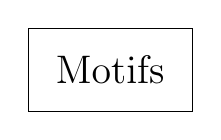
\begin{tikzpicture}
\node[draw,rectangle,inner sep=10pt] {\Large Motifs};
\end{tikzpicture}}

1) La catégorie $\mathcal{M}^+(X)$

2) Variance pour $X$

3) Cas $X=\varprojlim X_i$

4) Foncteurs $T_\ell$

5) Les $\mathbb{Q}_\ell(\unsure{+n|\pm n})$

6) La catégorie $\mathcal{M}(X)$

7) Les foncteurs $\operatorname{Hom}$ et $\operatorname{RHom}$

8) Motifs constants, tordus, et \unsure{pl. con.}

9) Filtrations de $\mathcal{M}(X)$ et $\mathcal{M}^+(X)$

10) Anneaux $\mathrm{M}^+(X)$ et $\mathrm{M}(X)$.

11) Interprétation topologique des
\deleted{\unsure{types d'isomotifs|types d'isomorphie}}\inserted{niveaux}
par la filtration canonique d'une variété proj. non singulière.

12) L'hom $L(k)\longrightarrow \mathrm{M}^+(k)$ et invariants birationnels fondamentaux.

[NB. À généraliser à des coefficients quelconques]

13) Caractérisation galoisienne des filtrations (conj. de Tate)

14) Invariants de Galois et homs de commutation.

15) Cohomologie absolue des motifs. Cas des schémas de type fini.

16) Relations avec les pts rationnels et la \unsure{cl.} des VA sur
un schéma de type fini.

17) Formes positives.

18) Motifs et fonctions $L$

19) Relations avec la cohomologie de Hodge \dots

\scanpage{23}
% Pencil foliation: 22, lower left.
\uline{Motifs}

1) À tout préschéma noeth (éventuellement de type fini sur un anneau
noethérien) $X$ est associé une \uline{catégorie abélienne}
$\mathcal{M}^+(X)$, dite catégorie des \uline{motifs} \inserted{\uline{effectifs}} sur $X$.
C'est une
$\mathbb{Q}$-catégorie \deleted{de $\mathbb{Q}$-modules} divisible, i.e. pour tt
$M\in\operatorname{Ob}\mathcal{M}^+(X)$ et $n\in\mathbb{Z}$, $n\ne0$,
$n\,\operatorname{id}_M$ est un isom
de $M$. De plus, $\mathcal{M}^+(X)$ est munie d'un
produit tensoriel commutatif et unitaire,
\inserted{(exact à droite,)}
l'unité est notée $\mathbf1_X$ ou $\mathbb{Q}_X(0)$

\margin{On peut en
termes des
\unsure{données} construire
des foncteurs
$\lambda^iM$ etc \dots}

On considère aussi la catégorie dérivée bornée
$D^b(\mathcal{M}^+(X))$ de $\mathcal{M}^+(X)$. Le produit tensoriel est
étendu en un bifoncteur $M$\uuline{$\otimes$}$N$ en $M,N\in D^b(\mathcal{M}^+(X))$

2) Soit $f:X\longrightarrow Y$ un morphisme de préschémas
\deleted{\unsure{loc}} noeth, il lui est associé un \uline{foncteur}
\uline{exact}
\diagram{\begin{tikzcd}
f^*:\mathcal{M}^+(Y)\arrow[r]&\mathcal{M}^+(X)
\end{tikzcd}}
compatible avec $\otimes$,
\inserted{d'où
\diagram{\begin{tikzcd}
Lf^*:D^b(\mathcal{M}^+(Y))\arrow[r]&D^b(\mathcal{M}^+(X)),
\end{tikzcd}}}
On a transitivité.
Si $f$ est de type fini, et propre \uline{ou} $Y$ excellent,
on \deleted{définit} a de \unsure{$=$|$\overline{\mathrm m}$} un foncteur
\diagram{\begin{tikzcd}
Rf_*:D^b(\mathcal{M}^+(X))\arrow[r]&D^b(\mathcal{M}^+(Y))
\end{tikzcd}}

\scanpage{24}
% Pencil foliation: 23, lower left.
satisfaisant une formule de transitivité,
et la formule de projection
\[
 Rf_*(M\otimes Lf^*(N))\simeq Rf_*(M)\otimes N
\]
\margin{Considérer
aussi la formule
de dualité entre $Rf_*,f^*$,
et les foncteurs
$f^!,Rf_!$ et leurs
relations d'adjonction,
et enfin les
formules \illegible{2}
\unsure{changement} en foncteurs \dots}

3) Supposons $X=\varprojlim X_i$, système projectif
filtrant \unsure{en. affine|en affine}. Alors par les foncteurs
images inverses, on a
\[
 \mathcal{M}^+(X)\simeq\varinjlim_i \mathcal{M}^+(X_i)
\]
En particulier, si $X$ est de type fini
sur $S=\operatorname{Spec}(A)$, alors $X$ est limite des
préschémas $X_i$ de type fini sur $\mathbb{Z}$, et
la détermination de $\mathcal{M}^+(X)$ avec ses
structures déjà envisagées est \deleted{\unsure{tout}} ramenée
au cas des préschémas de type fini.

De \unsure{$=$|$\overline{\mathrm m}$}, si $(S_i)$ est système
projectif filtré en affines, $S=\varprojlim S_i$,
et si $X,Y$ de t. f. sur $S$ sont
définis par $(X_i),(Y_i)$ de la
façon habituelle, si on prend des

\scanpage{25}
% Pencil foliation: 24, lower left.
$M_{i_0}\in\operatorname{Ob}D^b(\mathcal{M}^+(X_{i_0}))$, d'où $M_i,M$, on
aura pour $f_{i_0}:X_{i_0}\unsure{-|\longrightarrow}Y_{i_0}$ la relation
\[
 Rf_*(M)=\varinjlim_i v_i^*(Rf_{i*}(M_i))
\]
où $v_i:Y\unsure{-|\longrightarrow}Y_i$ est le morphisme
canonique.

4) Soit $\ell\in\mathbb{P}$ tel que $\ell\,1_X\in\Gamma(X,\mathcal O_X)$ soit
inversible. Alors on a un foncteur
\diagram{\begin{tikzcd}
T_\ell=T_\ell^{(X)}:\mathcal{M}^+(X)\arrow[r]&\mathcal{M}_\ell^+(X)
\end{tikzcd}}
où $\unsure{\mathcal{M}_\ell^*(X)|\mathcal{M}_\ell^+(X)}$ est \inserted{la catégorie}
formée des ``$\mathbb{Q}_\ell$-modules
constructibles sur $X$'', i.e. la catégorie
déduite de la catégorie des ``systèmes
$\ell$-adiques de faisceaux de $\ell$-torsion
constructibles'' en négligeant précisément
les faisceaux de torsion.
Le foncteur
$T_\ell$ est \inserted{\uuline{compatible avec} $\otimes$ \uuline{et unité}}
\uuline{exact} et \fbox{\uuline{fidèle}} (mais non
pleinement fidèle), \uuline{compatible avec le}

\scanpage{26}
% Pencil foliation: 25, lower left.
\uuline{changement de base} $f^*$, \uuline{et compatible}
\uuline{également avec} $Rf_*$
[N.B. $T_\ell$ s'étend
évidemment en un foncteur
\diagram{\begin{tikzcd}
D^b(\mathcal{M}(X))\arrow[r,dash]&D^b(\mathcal{M}_\ell(X))
\end{tikzcd}}].
\unsure{$\{$} La détermination
des $T_\ell$ est encore ramenée au cas où
$X$ est de t. f. sur $\mathbb{Z}$.

\margin{compatible
avec $f^!$,
$Rf_!$, avec l'hom
\unsure{interne} etc \dots}

\margin{\uline{NB.} Ceci
exclut déjà
le choix \uline{trivial}
$\mathcal{M}^+(X)=0$ pour tt
$X$, car il
faudrait qu'on
ait $R^*f_*(\mathbb{Z}_\ell)=0$
pour $f,\ell$, ce
qui n'est
pas vrai
en général \dots}

\deleted{Si $X$ est un $\mathbb{Q}$-schéma
\inserted{de \deleted{\unsure{présentation}}\inserted{type} fini,}
alors on
aussi un foncteur
\diagram{\begin{tikzcd}
T_\infty=T_\infty^{(X)}:D^b(\mathcal{M}(X))\arrow[r]&\mathcal{M}_\infty(X)
\end{tikzcd}}
$\mathcal{M}_\infty(X)$ est la catégorie des \inserted{$\mathcal O_X$-}Modules
cohérents. Le foncteur $T_\infty$ est encore
\uline{exact} et \uline{fidèle}, compatible avec
$f^*$ et $Rf_*$.}

\margin{\uline{Signaler aussi la}
\uline{compatibilité de $T_\ell$ avec}
\uline{l'isom. de Künneth}}

5) Pour tout $X$, on a un \deleted{\unsure{un}}
élément canonique
\[
 \unsure{\mathbb{Q}|\mathbb{Z}}_X(-1)\ \text{ou }\mathbf1_X(-1)\in\operatorname{Ob}\mathcal{M}^+(X)
\]

\scanpage{27}
% Pencil foliation: 26, lower left.
dont la formation est compatible avec chgt
de base (il suffit donc de le construire
sur $\operatorname{Spec}\mathbb{Z}$), avec \deleted{des} isom
\[
 T_\ell(\unsure{\mathbb{Q}|\mathbb{Z}}(\unsure{-1|1}))
 \simeq \unsure{\mathbb{Q}|\mathbb{Z}}_\ell(\unsure{-1|1})
 =\underbrace{T_\ell(\mathbb{G}_{\mathrm m})^{-1}}_{
 \substack{\text{Module de Tate}\\\text{\inserted{inverse} de }\mathbb{G}_{\mathrm m}}}
\]
et le cas échéant ($X$ sur $\mathbb{Q}$).

On peut définir $\unsure{\mathbb{Q}|\mathbb{Z}}(-1)$ comme
$R^2f_*(\deleted{\unsure{\mathbb{Z}}}\mathbf1_{\mathbb{P}^1_X})$,
où $f:\mathbb{P}^1_X\longrightarrow X$ est la
projection canonique. Posant
\[
 \unsure{\mathbb{Q}|\mathbb{Z}}(-n)=\unsure{\mathbb{Q}|\mathbb{Z}}(-1)^{\otimes n}
 \qquad\text{pour }n\ge0
\]
on peut prouver, à l'aide des
axiomes déjà posés, que si $f:X\unsure{-|\longrightarrow}S$
est \inserted{lisse} projectif à fibres \inserted{géom.} connexes non vides,
\deleted{partout} de dim relative $d$, alors
\[
 R^{2d}f_*(\mathbf1_X)\simeq\mathbb{Z}_S(-d)
\]
et si on enlève l'hyp. ``projectif'' mais
suppose $f$ quasi-projectif, on trouve encore
\[
 R^{2d}f_!(\mathbf1_X)\simeq\mathbb{Z}_S(-d)
\]

\scanpage{28}
% Pencil archive foliation: 27.
On \deleted{aura}\inserted{aura} de plus \deleted{compatibilité, \illegible{1}} si $X/S$ est
lisse et $Y\underset{i}{\subset}X$ est lisse sur $S$, de codim
$d$ dans $X$, l'isom
\[
Ri^!(\mathbf1_X)\simeq \unsure{\mathbb{Q}|\mathbb{Z}}_Y(-d)
\]
compatible avec les isom déjà connus
du point de vue $\ell$-adique \ldots

6) \deleted{Chaque $\mathcal{M}(X)$ est plongé dans}
Le foncteur
\[
M\unsure{\rightsquigarrow|\longmapsto}M(\unsure{-1|+1})=M\otimes\unsure{\mathbb{Q}|\mathbb{Z}}(+1)
\]
de $\mathcal{M}^+(X)$ dans lui-\unsure{$=$|$\overline{\mathrm m}$} est \uline{pleinement fidèle}
mais pas une équivalence en général.
Il y a donc une façon canonique
d'élargir $\mathcal{M}^+(X)$ en \deleted{$\mathcal{M}$}$\mathcal{M}(X)$ de telle façon
que $\otimes\unsure{\mathbb{Q}|\mathbb{Z}}(-1)$ devienne une équivalence,
en prenant la \inserted{pseudo-}limite inductive
\[
\mathcal{M}^+\xrightarrow{\otimes\unsure{\mathbb{Q}|\mathbb{Z}}(-1)}\mathcal{M}^+
\xrightarrow{\otimes\unsure{\mathbb{Q}|\mathbb{Z}}(-1)}\mathcal{M}^+.
\]
\margin{$\mathcal{M}^+(X)$ est une \uline{sous-catégorie abélienne épaisse de} $\mathcal{M}(X)$ ;
[\unsure{l'appart.} à $\mathcal{M}^+(X)$ se vérifie fibre par fibre]}
On prolonge
à $\mathcal{M}(X)$ la structure $\otimes$, donc $\unsure{\mathbb{Q}|\mathbb{Z}}(-1)$
devient inversible, de $\unsure{\mathbb{Q}|\mathbb{Z}}(1)$ pour inverse, et
tt élément de $\mathcal{M}(X)$ peut s'écrire pour

\scanpage{29}
% Pencil archive foliation: 28.
$n$ assez grand, sous la forme
$M_n(n)$, avec $M_n\in\operatorname{Ob}\mathcal{M}^+(X)$, [pour $n$ fixé,
$M_n$ est bien déterminé par $M$ à isom unique
près, et
\[
(M_n(n)\simeq M_{n+1}(n+1))\Longleftrightarrow(M_{n+1}\simeq M_n(-1)),
\]
on retrouve la description de $\mathcal{M}(X)$ en
termes de \unsure{pseudo-}$\underset{\longrightarrow}{\lim}$.]
Les foncteurs
$T_\ell$ s'étendent à $\mathcal{M}(X)$, de façon unique, de façon
à rester compatible avec $\otimes$.

7) Dans $\mathcal{M}(X)$, on a aussi des foncteurs
$\underline{\operatorname{Hom}}$, liés à $\otimes$ par la formule
habituelle
\[
\operatorname{Hom}(P\otimes Q,R)\simeq
\operatorname{Hom}(P,\underline{\operatorname{Hom}}(Q,R))
\simeq\operatorname{Hom}(Q,\underline{\operatorname{Hom}}(P,R)),
\]
et \deleted{satisfaisant}\inserted{qui s'étendent en}
\[
R\operatorname{Hom}(\unsure{P|R},Q)
\qquad P,Q\in\operatorname{Ob}D^bM(X)
\]
satisfaisant à la relation analogue
relativement à $\underline{\otimes}$.
\uuline{La formation des $\underline{\operatorname{Hom}}$
\inserted{et $R\underline{\operatorname{Hom}}$}
est compatible avec les} $T_\ell$.

\deleted{NB} [NB. On retrouve la formation
des $f^!$ \ldots]

\scanpage{30}
% Pencil archive foliation: 29.
8) Soient $\ell,\ell'\in\mathbb{P}$ premiers aux car rés.
de $X$. Soit $M\in\operatorname{Ob}\mathcal{M}^+(X)$. On veut
que
\[
\begin{array}{c}
T_\ell(M)\ \text{faisceau constant tordu}\\
\Updownarrow\\
T_{\ell'}(M)\ \text{faisceau constant tordu}
\end{array}
\]
et que sous ces conditions, $T_\ell(M)$ et
$T_{\ell'}(M)$ doivent avoir \unsure{$=$|$\overline{\mathrm m}$} rang en chaque
pt. Pour vérifier l'égalité des rangs, on
est ramené au cas où $X$ est \inserted{le} spectre d'un
corps (\unsure{fini} si on veut, \deleted{\unsure{à}} ou clôture alg.
d'un tel). Plus généralement, si
$u$ est un endomorphisme de $M$,
($X=\operatorname{Spec}k$, $k$ un corps), on en déduit
\[
T_\ell(u)\in\operatorname{End}T_\ell(M),\qquad
T_{\ell'}(u)\in\operatorname{End}(T_{\ell'}(M))
\]
et je dis qu'on a
\[
\boxed{\operatorname{Tr}T_\ell(u)=\operatorname{Tr}T_{\unsure{\ell|\ell'}}(u)
\in\mathbb{Q}}
\]
d'où, remplaçant $u$ par $\unsure{\bigwedge^i u|\lambda^i u}$, le fait
\[
\boxed{P(T_\ell(u),t)=P(T_{\ell'}(u),t)\in\mathbb{Q}[t]}
\]

\scanpage{31}
% Pencil archive foliation: 30.
[où il s'agit des polynômes caractéristiques]
Pour ceci, notons que
\[
u\in\operatorname{Hom}(\mathbf1_X,\operatorname{Hom}(M,M))
=\operatorname{Hom}(\mathbf1_X,\check M\otimes M)
\]
et on a un morphisme \uline{contraction}
\[
\check M\otimes M\longrightarrow\mathbf1_X
\]
\margin{\uline{à inclure dans le formalisme tensoriel}}
d'où un $c(u)\in\operatorname{Hom}(\mathbf1_X,\mathbf1_X)$
et \deleted{\unsure{on}} $\operatorname{Tr}T_\ell(u)=T_\ell(c(u))\in\mathbb{Q}_\ell$
et il suffit de savoir :
\[
\boxed{X\ \text{connexe}\Longrightarrow
\operatorname{Hom}(\mathbf1_X,\mathbf1_X)\simeq\mathbb{Q}\operatorname{id}_{\mathbf1_X}}
\]

9) \uline{Filtration de} $\mathcal{M}^+(X)$ \uline{et} $\mathcal{M}(X)$

\unsure{a)|1°)} \uline{Filtration par le poids},
\deleted{\unsure{W}}
\[
\deleted{\unsure{\mathcal{M}^+(X)}}\quad
\mathcal{M}^{+0}(X)\subset \mathcal{M}^{+1}(X)\subset\cdots\subset \mathcal{M}^{+i}(X)\subset\cdots
\]
\margin{indices en bas}
filtration \uline{exhaustive} de $\mathcal{M}^+(X)$. [L'appartenance
à $\mathcal{M}_i^+(X)$ se vérifie fibre par fibre,
\deleted{\unsure{Rappelons}}\deleted{les}
\inserted{(géométriques si on veut)}
et dans le cas $X$ de t.f. \inserted{sur $\mathbb{Z}$} il suffit de
vérifier en les pts fermés. (Pour ceux-
ci, il y a un critère par Frobenius, cf

\scanpage{32}
% Pencil archive foliation: 31.
plus bas).]
\margin{\deleted{bon pour}}
\deleted{$\mathcal{M}^i(X)$ est ``engendré'' par les
$R^if_*$ L'appartenance à $\mathcal{M}^i(\unsure{k(x)|X})$ de
$M|_x$ implique \unsure{que}}
Compatible aux
$f^*$, et \deleted{l'appart.}
\[
M|_x\in\operatorname{Ob}\mathcal{M}^{+i}(k(x))
\Longrightarrow
\exists U\ni x\ \text{voisinage de $\bar{x}$, tel que }
M|_U\in\operatorname{Ob}\mathcal{M}^{+i}(U).
\]
\margin{\unsure{quasi-limite} Compatibilité aux $\underset{\longleftarrow}{\lim}$ de préschémas \ldots}
Soit $f:X\unsure{-|\longrightarrow}Y$,
alors
\[
R^jf_!:\mathcal{M}^{+i}(X)\longrightarrow \mathcal{M}^{+i+j}(Y);
\]
de plus, $\mathcal{M}^{+i}(k)$ ($k$ un corps alg. clos)
est ``engendré'' par les \inserted{sous-quotients}
$R^jf_!(\deleted{\mathbb{Z}}\mathbf1_X)$ pour
$X$ \unsure{disons} projectif lisse de dim $\leq j$ sur $k$
[au sens que tout $M\in\operatorname{Ob}\mathcal{M}^i(k)$ a une
filtration dont les facteurs sont isomorphes
à de tels sous-quotients].
\margin{indices en bas}
\[
\deleted{\mathcal{M}^i(X)\otimes\mathbb{Z}(-1)}
\]
\[
\left\{
\begin{array}{l}
\mathcal{M}_i^+(X)\otimes \mathcal{M}_j^+(X)\subset \mathcal{M}_{i+j}^+(X)\\
\mathbb{Z}(-1)\in\operatorname{Ob}\mathcal{M}_2^+(X)
\end{array}\right.
\]
d'où
\[
\mathcal{M}^{+i}(X)\otimes\mathbb{Z}(-j)\subset \mathcal{M}^{+i+2j}(X)
\qquad\text{pour }j\geq0
\]

\scanpage{33}
% Pencil archive foliation: 32.
on a mieux :
\[
M\in\operatorname{Ob}\mathcal{M}_i^+(X)\Longleftrightarrow
M(-j)\in\operatorname{Ob}\mathcal{M}^{+i+2j}(X)
\]
De cette façon, la filtration \inserted{de $\mathcal{M}^+(X)$} par les
$\mathcal{M}_i^+(X)$ \inserted{($i\geq0$)} peut se prolonger en une filtration
de $\mathcal{M}(X)$ par des $\mathcal{M}^i(X)$ ($i\in\mathbb{Z}$) de
telle façon que pour $i\geq0$, on ait la filtration
déjà \deleted{\unsure{\mathcal{M}^+(X)}} envisagée, et pour $i$ quelconque,
on définit
\[
M\in\operatorname{Ob}\mathcal{M}^i(X)\Longleftrightarrow
M(-j)\in\operatorname{Ob}\mathcal{M}^{i+2j}(X)
\]
si on prend $j$ assez grand pour que
$M(-j)\in\operatorname{Ob}\mathcal{M}^+(X)$. On notera que
\[
\mathcal{M}^{+i}(X)=\mathcal{M}^i(X)\cap \mathcal{M}^+(X)
\]
\margin{indices en bas}
si $i\geq0$, et pour tt $i$ si on définit
\[
\mathcal{M}^{+i}(X)=\{0\}\deleted{\unsure{\mathcal{M}^+(X)}}\quad\text{si }i<0
\]
\deleted{(\unsure{on voit} par là \illegible{3} que $\mathcal{M}^{+i}(X)$
\inserted{\deleted{$\mathcal{M}^+(X)$}}
\unsure{croisse avec $i$})}
On aura
\[
\otimes\unsure{\mathbb{Q}|\mathbb{Z}}(-1):
\mathcal{M}^i(X)\overset{\text{équiv}}{\simeq}\mathcal{M}^{i+2}(X)
\]
\[
\otimes\unsure{\mathbb{Q}|\mathbb{Z}}(j):
\mathcal{M}^i(X)\overset{\text{équiv}}{\simeq}\mathcal{M}^{i-2j}(X)
\]

\scanpage{34}
% Pencil archive foliation: 33.
mais on fera attention que l'inclusion
\[
\unsure{\mathbb{Q}|\mathbb{Z}}(-1)\otimes \mathcal{M}^{+i}(X)
\hookrightarrow \mathcal{M}^{+(i+2)}(X)
\]
plus gén.
\[
\unsure{\mathbb{Q}|\mathbb{Z}}(-j)\otimes \mathcal{M}^{+i}(X)
\subset \mathcal{M}^{+(i+2j)}(X)
\]
est \uline{stricte} en général, i.e. n'est pas
une équivalence de catégories.

Noter que $\mathcal{M}^{+i}(X)$ est \uline{épaisse} dans $\mathcal{M}^{+j}(X)$
\margin{indices en bas}
\deleted{[elle est définie dans la catégorie}, et de
\unsure{$=$|$\overline{\mathrm m}$} $\mathcal{M}^i(X)$ épaisse dans $\mathcal{M}^j(X)$ $(i\leq j)$.
Les quotients
\[
\inserted{C_i^+(X)=}
\operatorname{Gr}_i^{\unsure{F|\varepsilon}}(\mathcal{M}^+(X))
\deleted{\unsure{\mathord{?}}}
\inserted{\simeq \mathcal{M}_i^+(X)/\mathcal{M}_{i-1}^+(X)}
\quad\text{et}\quad
C_i(X)=\operatorname{Gr}_i^{\unsure{F|\varepsilon}}(\mathcal{M}(X))
\simeq \mathcal{M}_i(X)/\mathcal{M}_{i-1}(X)
\]
sont fort intéressants.
Noter que les $\unsure{C_i(X)|C_{2i}(X)}$ sont tous
\deleted{isomorphes}\inserted{équivalents}
par twisting
\[
C_i(X)\overset{\mathbb{Z}(-j)}{\simeq}C_{i+2j}(X),
\]
en particulier tous \deleted{isomorphes}\inserted{équiv. can.} à $C_0(X)$.
D'ailleurs
\[
C_i^+(X)\underset{\sim}{\subset}C_i(X)\simeq C_0(X)
\]
\inserted{équiv. à une} sous-catégorie pleine et \uline{épaisse} de
$C_i(X)\simeq C_0(X)$.

\scanpage{35}
% Pencil archive foliation: 34.
b) Filtration par \deleted{``la dimension''} ``type dimensionnel''.

On pose pour $i\geq0$
\[
D_i(\mathcal{M}^+(X))=
\deleted{\unsure{\mathcal{M}}}\text{sous-catégorie pleine}
\]
de $\mathcal{M}^+(X)$, formée des objets
qui se \inserted{loc étale} dévissent [(au moins,
fibre par fibre)] en objets
de la forme
\margin{\deleted{\unsure{NB}}}
\[
\deleted{\unsure{\longrightarrow}}\quad
M(-j),\quad\text{avec }M\in\operatorname{Ob}\mathcal{M}^{+i}(X),\quad
j\in\mathbb{Z},\ j\geq0
\]
i.e. on prend (du moins pour $X=\operatorname{Spec}K$ d'un
corps) la filtration minimum qui
majore celle par le poids, \deleted{\illegible{1}} qui est
stable par $\otimes\unsure{\mathbb{Q}|\mathbb{Z}}(-1)$, et \uline{épaisse}.

Les $D_i(\mathcal{M}^+(X))$ sont stables par l'image inverse,
et pour l'image directe on a
\[
R^jf_!(D_i(\mathcal{M}^+(X)))\subset D_{i+j}(\mathcal{M}^+(Y))
\]
\[
R^jf_*(D_i(\mathcal{M}^+(X)))\subset D_{i+j}(\mathcal{M}^+(Y))
\]
\margin{\figure{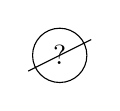
\begin{tikzpicture}
\node[draw,circle,inner sep=4pt] (q) at (0,0) {?};
\draw (-.4,-.2)--(.4,.2);
\end{tikzpicture}}}
\margin{\deleted{le cas critique est celui d'une immersion ouverte}}
\margin{cela distingue formellement les filtrations $D_i(\mathcal{M})$ et $\mathcal{M}_i$ !}
[On a seulement
$R^jf_*(\mathcal{M}^{+i}(X))\subset \mathcal{M}^{+(i+2j)}(Y)$ !?]
\margin{\figure{\begin{tikzpicture}
\node[draw,ellipse,align=center] {\unsure{tout formel|tout finit}\\
\unsure{en dessous de}\\
la dim. de $X$ !};
\end{tikzpicture}}}
On \deleted{\unsure{remarque}} a
\[
M\in\operatorname{Ob}D_i(\mathcal{M}^+(X))
\Longleftrightarrow
M(-j)\in\operatorname{Ob}D_{\unsure{i|i+j}}(\mathcal{M}^+(X))
\]
\margin{\figure{\begin{tikzpicture}
\node[draw,ellipse] (d) at (0,0) {$D_i$};
\node (r) at (3,1) {\uline{pas} $D_{i+j}$!!};
\draw[->] (d)--(r);
\end{tikzpicture}}}
et la filtration \inserted{de $\mathcal{M}^+(X)$} par les $D_i(\mathcal{M}^+(X))$ s'étend
en une filtration de $\mathcal{M}(X)$ par des $D_i(\mathcal{M}(X))$.

\scanpage{36}
% Pencil archive foliation: 35.
induisant la filtration donnée, \deleted{et on a}
\[
M\in\operatorname{Ob}D_i(\mathcal{M}(X))\Longleftrightarrow
M(-j)\in\operatorname{Ob}D_i(\mathcal{M}(X))
\quad\text{pour }j\ \text{qque}
\]
\deleted{ici}
On a
\[
\deleted{D_i(\mathcal{M}^+(X))/D_{i-1}(\mathcal{M}^+(X))
\xrightarrow{\simeq}D_i(\mathcal{M}(X))/D_{i-1}(\mathcal{M}(X))}
\]
\[
D_i(\mathcal{M}(X))\otimes D_j(\mathcal{M}(X))\subset D_{i+j}(\mathcal{M}(X))
\]
\inserted{\[
\boxed{\text{mais }\mathbb{Z}(-j)\in\operatorname{Ob}D_0(\mathcal{M}(X))
\text{ pour tt }j.}
\]}
et de \unsure{$=$|$\overline{\mathrm m}$} en mettant des $+$.
Enfin, on a
\[
\underline{\underline{\operatorname{Ext}}}^{\unsure{i}}(D_j(\mathcal{M}(X)),D_k(\mathcal{M}(X)))
\subset D_{\unsure{j+k|i+j+k}}(\mathcal{M}(X))
\]
(pas de formule aussi simple en termes
des $\mathcal{M}_\alpha(X)$ !).

10) \uline{Motifs constants tordus}. \uline{Anneaux} $\mathrm{M}^+(X)$ et $\mathrm{M}(X)$

Soit $\mathcal{M}^+(X)_{\mathrm{spec.}}$ la ss-catégorie des
motifs effectifs \uline{constants tordus}.
[\deleted{\unsure{que}} condition locale, qui se vérifie sur
$T_\ell(M)$, cf N° 8], et de \unsure{$=$|$\overline{\mathrm m}$} on définit
$\mathcal{M}(X)_{\mathrm{spec.}}$ \deleted{Noter que $M$ est}
Ainsi
$M$ est tordu $\Longleftrightarrow M(j)$ est tordu.

$\mathcal{M}^+(X)_{\mathrm{spec.}}$ et $\mathcal{M}(X)_{\mathrm{spec.}}$ sont des
\inserted{ss-}\uline{catégories abéliennes},
\uline{stables par extensions}, \uline{dont tt objet est de}

\scanpage{37}
% Pencil archive foliation: 36.
\uuline{longueur finie}. Elle est stable par $\otimes$,
sur cette catégorie les $\operatorname{Ext}^i$ $(i>0)$ sont
nuls, et la catégorie est aussi stable
par $\operatorname{Hom}$ (cas de $\mathcal{M}(X)_{\mathrm{spec.}}$). On a
une ``catégorie tensorielle sur $\mathbb{Q}$''.

Le \deleted{\unsure{le|la}} $\lambda$-anneau défini par cette
catégorie est noté $\mathrm{M}^+(X)$ resp. $\mathrm{M}(X)$.
Noter que $\xi=\operatorname{cl}\text{ de }\unsure{\mathbb{Q}|\mathbb{Z}}_X(-1)$ est une
\unsure{droite} de $\mathrm{M}^+(X)$, et on a
\[
\mathrm{M}(X)=\mathrm{M}^+(X)_\xi=\mathrm{M}^+(X)\left[\frac1\xi\right].
\]
En fait, $\xi$ est non div. de $0$ :
$\mathrm{M}^+(X)$ comme $\mathbb{Z}$-module admet comme
base les classes d'\deleted{\uline{éléments}}\inserted{objets} \uline{simples} de
$\mathcal{M}^+(X)$, et $x\unsure{\rightsquigarrow|\mapsto}\xi.x$ dans $\mathrm{M}^+(X)$ est défini
par une application \uline{injective} sur l'ens des
objets simples. [N.B. $M$ simple \inserted{ds $\mathcal{M}^+(X)$}
$\Longleftrightarrow$ \inserted{$M$ simple dans $\mathcal{M}(X)\Longleftrightarrow$}
$M(-1)$ simple, comme il résulte du
fait que $\mathcal{M}^+(X)$ est épaisse dans $\mathcal{M}(X)$ et
$\otimes\mathbb{Z}(-1)$ une autoéquivalence.]

\scanpage{38}
% Pencil archive foliation: 37.
Si $\Sigma^+(X)=\text{ens des classes d'objets simples}$
de $\mathcal{M}^+(X)$,
\[
\Sigma(X)=\underset{\substack{\longrightarrow\\
\text{par }e\unsure{\rightsquigarrow|\mapsto}\xi e}}{\lim}\Sigma^+(X),
\]
on aura par \deleted{$\mathcal{M}(K)$} un diagramme comm.
\diagram{\begin{tikzcd}
\mathrm{M}^+(X) \arrow[d,hook] \arrow[r,equal] &
\mathbb{Z}^{(\Sigma^+(X))} \arrow[d,hook]\\
\mathrm{M}(X) \arrow[r,equal] &
\mathbb{Z}^{(\Sigma(X))}
\end{tikzcd}}
Alors $\mathcal{M}_i^+(X)$ est défini en termes
d'une partie $\Sigma_{(i)}^+(X)$ de
$\unsure{\Sigma_i(X)|\Sigma(X)}$,
d'où
\[
\mathrm{M}_i^+(X)=\mathbb{Z}^{\Sigma_{(i)}^+(X)}
\]
ce qui donne une filtration croissante
sur l'anneau $\mathrm{M}^+(X)$, et une
filtration analogue sur $\mathrm{M}(X)$.
En fait, posant
\[
\Sigma_i^+(X)=\Sigma_{(i)}^+(X)-\Sigma_{(i-1)}^+(X)
\]
on aura \unsure{$=$|$\overline{\mathrm m}$}
\[
\Sigma_i^+(X).\Sigma_j^+(X)\subset
\mathbb{Z}^{\Sigma_{i+j}^+(X)}
\]
donc $\mathrm{M}^+(X)$ devient un \uline{anneau}

\scanpage{39}
% Pencil archive foliation: 38.
\uline{gradué} \inserted{\uline{à degrés} $\geq0$}, et $\xi$ est de degré $1$. De cette
façon, $\mathrm{M}(X)$ devient gradué [à degrés
de tous signes, $\xi$ étant une \unsure{droite}
\uline{inversible} de degré $1$]. Noter que
\[
\mathrm{M}_0(X)\simeq\mathbb{Z}^{\Sigma_0(X)}
\]
avec
\[
\Sigma_0(X)=\underset{\substack{\longrightarrow\\
\text{par }x\unsure{\rightsquigarrow|\mapsto}x.\xi}}{\lim}\Sigma_i^+(X)
\]
et
\[
\mathrm{M}^{\mathrm{pair}}(X)=
\underbrace{\mathrm{M}_0(X)}_{\text{de degré }0}
[\underbrace{\xi}_{\text{de degré }1}]
\]
\inserted{\[
\mathrm{M}^{\mathrm{impair}}(X)=
\mathrm{M}_1(X)\otimes_{\mathrm{M}_0(X)}\mathrm{M}_0(X)[\xi]
\]}
donc la structure d'anneau gradué
de $\mathrm{M}(X)$ est déterminée en termes de
la structure d'anneau de $\mathrm{M}_0(X)$, \deleted{et}
du module $\mathrm{M}_1(X)$ sur $\mathrm{M}_0(X)$, et l'application de mult.
\inserted{définie par \deleted{\unsure{\xi}} $u,v\unsure{\rightsquigarrow|\mapsto}\xi^{-1}uv$.}
\[
\mathrm{M}_1(X)\otimes_{\mathrm{M}_0(X)}\mathrm{M}_1(X)
\longrightarrow\mathrm{M}_0(X)
\]

D'autre part les objets de $D_i^+(\mathcal{M}^+(X))$
sont \deleted{ceux qui}\inserted{ceux} dont la classe dans
\deleted{$\mathcal{M}^+(X)$ sont} $\mathrm{M}^+(X)$ sont dans
$\mathbb{Z}^{D_i(\Sigma^+(X))}$.
\[
\left.
\begin{aligned}
D_i(\Sigma^+(X))&=
\coprod_{j\geq0}\deleted{\unsure{\Sigma}}\xi^j\Sigma_{(i)}^+(X)\\
&=\coprod_{\substack{j\geq0\\0\leq k\leq i}}\xi^j\Sigma_k^+(X)
\end{aligned}
\right\}\Sigma_{[i]}^+(X)
\]

\scanpage{40}
% Pencil archive foliation: 39.
Posons
\[
\deleted{\unsure{\Sigma}}\ \sigma_i(X)=
\Sigma_i^+(X)-\bigcup_{\substack{\deleted{\unsure{\alpha<i}}\\\alpha\geq0}}
\xi^\alpha\Sigma_{i-2\alpha}^+(X).
\]
On a une partition (au sens large)
\[
\unsure{\Sigma_{2i}(X)|\Sigma_i^+(X)}
=\sigma_i(X)\cup\xi\sigma_{i-2}(X)\cup\cdots\cup
\left\{\begin{array}{l}
\xi^{i/2}\sigma_0(X)\\
\xi^{(i-1)/2}\sigma_1(X)
\end{array}\right.
\]
\margin{\deleted{\unsure{$i$ pair} \unsure{$i$ impair}}}
\margin{\figure{\begin{tikzpicture}
\node[draw,ellipse,align=center] {éléments\\\uline{primitifs}\\de poids $i$};
\end{tikzpicture}}}
et on a donc
\[
D_i(\Sigma^+(X))\cap\Sigma_j^+(X)=
\left\{\begin{array}{ll}
\Sigma_j^+(X)&\text{si }j\leq i\\
\deleted{\unsure{\xi}}\xi^{j-i}\sigma_i(X)\cup
\xi^{j-i-1}\sigma_{i-1}(X)\cup\cdots\cup\xi^j\sigma_0(X)
&\text{si }j>i
\end{array}\right.
\]
Ainsi
\[
\begin{aligned}
D_i(\mathrm{M}^+(X))/D_{i-1}(\mathrm{M}^+(X))
&\simeq\mathbb{Z}^{D_i(\Sigma^+(X))-D_{i-1}(\Sigma^+(X))}\\
&\simeq\mathbb{Z}^{\sigma_i(X)+\xi\sigma_{i-2}(X)+\xi^2\sigma_{i-4}(X)+\cdots}.
\end{aligned}
\]
\deleted{$\unsure{\mathbb{Z}^{\sigma_i(X)}}$}

\uline{N.B.} Du pt de vue de la structure additive,
des deux filtrations, et de l'opération
$\xi.$, $\mathrm{M}^+(X)$ et $\mathrm{M}(X)$ sont complètement
déterminés par la connaissance de
la famille $(\sigma_i(X))_{i\geq0}$ des \uline{ens} $\sigma_i(X)$.
Pour la structure multiplicative, il faut
connaître de plus les applications
\[
\sigma_i(X)\times\sigma_j(X)\longrightarrow
\mathbb{Z}_{\unsure{\sim|+}}^{\left(\coprod_{\unsure{k\leq i+j.2|k\equiv i+j,2}}
\sigma_k(X)\right)}
\]
\margin{définies par $\unsure{x,y|u,v}\rightsquigarrow\deleted{\unsure{\xi^{-1}}}uv$.}

\scanpage{41}
% Pencil archive foliation: 40.
Nous allons expliciter plus bas la détermination
de $\sigma^0(X)$ et $\sigma^1(X)$.

Il y a lieu également de préciser
les opérations $\vee$ et $\lambda^i$. Pour la
première, notons que
\[
\unsure{\mathbb{Q}|\mathbb{Z}}(-i)[\mathcal{M}_i^+(X)]^\vee\subset \mathcal{M}_i^+(X)
\]
d'où on conclut de proche en
proche que $x\unsure{\rightsquigarrow|\mapsto} \check x\xi^i$ définit sur
$\sigma_i$ une involution. Mais en fait il
résultera de la théorie \unsure{projetée|projective} que
\uline{cette dernière est l'identité}, i.e.
\uline{l'opération} $\vee$ \uline{dans} \deleted{\unsure{\mathcal M}}
$\mathrm{M}_i(X)$ \deleted{est l'identité} \uline{n'est
autre que} $x\unsure{\rightsquigarrow|\mapsto}\xi^{-i}x$,
\deleted{\unsure{donc dans} $\mathrm{M}(X)$
$x\unsure{\rightsquigarrow|\mapsto} \check x=\xi^{-i}x$}.
Quant aux opérations $\lambda^i$, leur détermination
devrait se faire en termes de groupes finis
d'opérateurs (tels les $\unsure{\mathfrak{S}_p|G_p}$ \ldots).

\scanpage{42}
% Pencil archive foliation: 41.
\uline{11} \uline{Interprétation topologique du type}
\deleted{\unsure{filtre}} \uline{dimensionnel} (Cas ``géométrique'').

Soit $X$ \deleted{projectif} non singulier sur $k$
alg. clos. Considérons la filtration $X$
par la codimension, et la suite spectrale
\[
H^n(X,\unsure{\mathbb{Q}|\mathbb{Z}}_\ell)
\Longleftarrow
\inserted{E_1^{pq}=}
\coprod_{x\in X[p]}H^{q-p}(x,\unsure{\mathbb{Q}|\mathbb{Z}}_\ell(-p))
\deleted{\unsure{\xi}}
\]
\margin{Attention aux \unsure{infinis} $E_1$ et $E_2$ !!}
où on pose
\[
\left\{\begin{array}{l}
X[p]=\{x\in X\mid\dim\mathcal{O}_{X,x}=p\}\\
H^\alpha(x,\mathbb{Z}_\ell(-p))=
\underset{\substack{\longrightarrow\\
U\text{ ouvert }\ne\varnothing\text{ de }\bar{x}}}{\lim}
H^\alpha(U,\unsure{\mathbb{Q}|\mathbb{Z}}_\ell(\unsure{-p|p})))
\end{array}\right.
\]
\figure{\begin{tikzpicture}
\draw (-.4,0)--(3.2,0);
\draw (0,-.4)--(0,2.6);
\draw (0,0)--(3.2,2.5);
\node at (3.6,0) {$p$};
\node at (-.2,2.7) {$q$};
\node at (2.7,1.1) {$0$};
\end{tikzpicture}}
On veut que \deleted{la \unsure{provenance de}} cette suite spectrale
provienne d'une suite spectrale de
motifs (du moins à partir de $E_r^{pq}$ avec
$r\geq2$ ; sinon il faudrait parler de
ind-motifs, ou bien prendre une
filtration \uline{finie} convenable de $X$ par des
sous-schémas fermés].
\margin{\unsure{codim $p$|en dim $p$}}
Le morceau
de la filtration $\geq p$ est visiblement de
type dimensionnel $\leq n-2p$. On veut que
ce soit \uline{exactement} le morceau de type
dimensionnel $n-p$.
\margin{si $X$ est \uuline{\uline{projectif}}
(\unsure{l'hypothèse essentielle}, \unsure{penser}
à $X$ de dim $1$ !)}

\figure{\begin{tikzpicture}
\draw (0,1.2)--(0,.15) .. controls (-.16,.05) and (-.16,-.13) .. (0,-.08) .. controls (.12,-.03) and (.13,.13) .. (0,.15);
\draw (6,1.2)--(5.95,.15) .. controls (5.78,.07) and (5.78,-.10) .. (5.94,-.07) .. controls (6.09,-.02) and (6.09,.13) .. (5.95,.15);
\end{tikzpicture}}

\scanpage{43}
% Pencil archive foliation: 42.
\deleted{
si le \unsure{fais.} motif de coefficient $\mathbb{Z}(0)$
est remplacé par un motif constant
tordu de \inserted{pur} type dimensionnel \deleted{de} $\delta$
[Attention au décalage par $\delta$ !]. Cet
énoncé \deleted{est un} \uline{\unsure{précise|précède}} les interprétations
galoisiennes et la conjecture de Tate
des \unsure{problèmes}, et est sans doute moins
profond.
}
\margin{\deleted{
$X$ de dim $n$, $U$ ouvert, $X-U$ de dim $<n$.
Alors si \unsure{$i\leq n$}, $H^i(X)\deleted{\unsure{\simeq}}\unsure{\longrightarrow|-}H^i(U)$
est un isom \uuline{mod}
$D_{\unsure{i-1}}(\mathcal{M}^+(K))$, donc $H^i(X)$ et
$H^i(U)$ ont \unsure{$=$|$\overline{\mathrm m}$} composant dans
$D_{\unsure{i|n}}(\mathcal{M}^+(K))/D_{\unsure{i-1|n-1}}(\mathcal{M}^+(K))$.
De plus (via résolution) ce dernier est dans
l'image de $\mathcal{M}_i^+(K)$, d'où un inv. birationnel
$\in\mathbb{Z}^{\unsure{\sigma_i}}\ldots$
}}

\unsure{12)} \deleted{\unsure{B.}}
\uline{L'hom fondamental}
\[
L(K)\unsure{-|\longrightarrow}\mathrm{M}^+(K)
\]
\uline{et invariants birationnels fondamentaux}.

$K$ est un corps. On désigne par
$L(K)$ le gpe \unsure{$K$} engendré par les
préschémas de type fini sur $K$, avec
comme relations celles définies par
découpage en morceaux. C'est un
anneau par $\otimes$. On définit
un hom d'anneaux
\[
\sigma:L(K)\longrightarrow\mathrm{M}^+(K)
\]

\scanpage{44}
% Pencil archive foliation: 43.
par
\[
\operatorname{cl}(X)\unsure{\rightsquigarrow|\longmapsto}
\sum(-1)^i\operatorname{cl}H_!^i(X,\unsure{\mathbb{Q}|\mathbb{Z}}(0))
\]
où bien entendu $H_!^i(X,\mathbb{Z}(0))$ est
\deleted{considéré}\inserted{défini} comme motif sur $K$ par
$R^if_!(\unsure{\mathbb{Q}|\mathbb{Z}}(0))$ ;
$f:X\unsure{-|\longrightarrow}\operatorname{Spec}K$ la projection.
Prenant les composantes homogènes de
$\sigma\operatorname{cl}(X)$, on a des $\sigma_i(\operatorname{cl}(X))$ qui sont
des ``motifs virtuels'', et permettent de
définir des ``nbs de Betti virtuels'', ceux
demandés par Serre.

\deleted{
Si on filtre $L(K)$ par la dimension
en des $L_i(K)$, on trouve
\[
L_i(K)\longrightarrow D_i(\mathrm{M}^+_{\unsure{\ell|{}}}(K))
\]
On peut se demander si c'est surjectif,
ou injectif, \deleted{bijectif serait étonnant}
\unsure{même} mod torsion. Déjà pour $i=1$
($K$ alg clos) \inserted{\unsure{si le} degré de trans. infini du corps de base},
rien n'est connu.
On peut poser la question en
considérant des $X/K$ munis d'un groupe fini
donné $G$ d'autom. --- mais il faut
}
\margin{\deleted{
Pb pas bien \unsure{posé} car \unsure{aucune}
\unsure{définition} \uline{\unsure{rigide|rigidité}} \unsure{à|et}
telle quelle. cf plus bas la formulation
correcte \ldots
En fait
\[
L_i(K)\longrightarrow
\mathrm{M}_{(i)}^+(K)+\xi\mathrm{M}_{(i-1)}^+(K)
+\xi^2\mathrm{M}_{(i-2)}^+(K)+\cdots
\]
}}

\scanpage{45}
% Pencil archival foliation: 44.
Filtrons $L(K)$ par la dimension, on trouve
\[
L_{(i)}(K)\longrightarrow
\underbrace{
\begin{array}{ccccc}
\mathrm{M}^{+}_{(i)}(K)&+\xi\,\mathrm{M}^{+}_{(i-1)}(K)&+\xi^n\mathrm{M}^{+}_{(i-n)}(K)&+\cdots\\
&\cap&\cap\\
&\mathrm{M}^{+}_{i+1}(K)&\uline{\mathrm{M}}^{+}_{i+n}(K)
\end{array}}_{=\,D'_i(\mathrm{M}^{+}(K))}
\]
\deleted{\unsure{d'où} si $X\in$}
\margin{\deleted{\unsure{NB}}}

d'où un hom. naturel
\diagram{\begin{tikzcd}
\operatorname{gr}_n(L(K))\arrow[r]&
\operatorname{gr}'_{\unsure{n}}(\mathrm{M}^{+}(K))\arrow[d,equal]\\
&\mathbb{Z}^{\deleted{\unsure{E}}(\sigma_n\cup\xi\sigma_{n-1}\cup\xi^2\sigma_{n-2}\cup\cdots)}
\end{tikzcd}}
\margin{filtration par les $D'_i(\mathrm{M}^{+}(K))$}
Donc, si $X$ est un préschéma de type
fini \deleted{de} sur $K$, de dim $\leq n$, en
prenant $\operatorname{cl}(X)\in L_n(K)$ et réduisant
modulo $L_{n-1}(K)$, on trouve une image
dans $\mathbb{Z}^{(\sigma_n\cup\xi\sigma_{n-1}\cup\cdots)}$ donc un
invariant de la forme
\[
\gamma_n(X)+\xi\gamma_{n-1}(X)+\xi^2\unsure{\gamma_{n-2}(X)}+\cdots
\]
\deleted{
\[
\unsure{\beta_n(X)|\gamma_n(X)}
+\xi\beta_{n-1}(X)+\xi^2\beta_{n-2}\unsure{(X)}+\cdots
\]
\uline{poids} \unsure{resp.} $n\qquad n+1\qquad n+2$
}
\inserted{[poids $n,\ n+1,\ n+2,\ldots$]}

\scanpage{46}
% Pencil archival foliation: 45.
où disons
\[
\unsure{\gamma_j(X)|\beta_j(X)}\in\mathbb{Z}^{\sigma_j(X)}
\qquad 0\leq j\leq n
\]
Ils sont obtenus en prenant les
$\beta_k(X)$ de Serre [composants de poids purs
de $\operatorname{cl}(X)$] pour $k\geq n$, et \deleted{les composant}
\inserted{en notant}
qu'un tel $\beta_k(X)$ se met sous la forme
\[
\xi^{k-n}\unsure{\beta'_{2n-k}(X)},\quad\text{où}\quad
\unsure{\beta'_{2n-k}(X)}\in\mathrm{M}^{+}_{2n-k}(K);
\]
alors $\gamma_{2n-k}(X)$ s'obtient en prenant la composante
\uline{bipure} de $\unsure{\beta'_{2n-k}(X)}$ ----- .
\margin{\figure{\begin{tikzpicture}
\node[draw,ellipse,align=center] {\unsure{au signe}\\près!};
\end{tikzpicture}}}

Par construction \unsure{$=$|$\overline{\mathrm m}$}, les invariants
ainsi obtenus sont des invariants
$n$-birationnels de $X$. Si $X$ est projective
\uline{lisse sur $K$}\deleted{\unsure{la condition}}, les $\beta'_j(X)$ pour $0\leq j\leq n$
n'est autre (par \uuline{Lefschetz}\ldots) que
la classe des $H^j(X,\unsure{\mathbb{Q}(0)|\mathbb{Z}(0)})$. Donc notre construction
consiste à prendre la composante bipure des
$H^j(X,\unsure{\mathbb{Q}(0)|\mathbb{Z}(0)})$. Mais cela n'est autre aussi.

\scanpage{47}
% Pencil archival foliation: 46.
d'après le n° précédent que \deleted{la composante \unsure{bipure} de}
\inserted{l'image dans}
\[
\varinjlim_{\substack{U\ \mathrm{ouvert}\\ \deleted{\mathrm{de}}\\ \mathrm{dense}}}
H^j(U,\unsure{\mathbb{Q}(0)|\mathbb{Z}(0)})
\]
de $H^j(X,\mathbb{Z}(0))$.

En fait, on constate (via dualité)
que si $X$ est lisse (sans doute
inutile) de dim $\leq n$, et si $i\leq n$
alors pour $\forall$ ouvert dense $U$ de $X$,
\[
H^i(X)\unsure{-|\longrightarrow}H^i(U)
\]
est \uline{\deleted{bijectif}\inserted{injectif} mod}
$D_{i-2}(\mathcal{M}^{+}(X))$ et
\uline{bijectif mod $D_{i-1}(\mathcal{M}^{+}(X))$}; ce qui
donne un invariant birationnel dans
\[
D_i(\mathcal{M}^{+}(X))/\unsure{D_{i-1}}(\mathcal{M}^{+}(X)),
\]
lequel
est d'ailleurs dans l'image de
$\mathcal{M}^{+}_{(i)}(X)$, donc définit un objet de
\[
\mathcal{M}^{+}_{(i)}(X)/
[\mathcal{M}^{+}_{(i-1)}(X)\unsure{+}\xi\mathcal{M}^{+}_{(i-2)}(X)],
\]
donc un
élément de $\mathbb{Z}^{\sigma_i(X)}$. C'est
l'invariant birationnel $\gamma_i(X)$.

\scanpage{48}
% Pencil archival foliation: 47.
Sous la forme précédente, on voit que
l'on a mieux que \deleted{des} \unsure{invariants|invariant}
dans $\mathrm{M}^{+}_i(K)$. En fait, on a des
\[
\underline{\gamma}^{\,i}(X)\in
\operatorname{Ob}\mathcal{M}^{+}_{i\ \mathrm{bipur}}(K),
\]
objets semi-simples;
définis de la façon suivante ($K$ parfait,
ce qu'on peut supposer)
\inserted{$\gamma^i(X)\unsure{\subset|\in}
\varinjlim_{U\ \mathrm{ouvert\ dense}}H^i(U,\mathbb{Z}(0))$}
est le plus grand sous-motif \uline{bipur} de
type $i$.
\deleted{[Ainsi le foncteur $\unsure{\gamma^i(X)}$}
\inserted{C'est un foncteur en $X$}
[\unsure{via|si on} \unsure{l'anneau} des fonctions rat. sur $X$,
comme sp. sur $K$], de façon évidente
\margin{\diagram{\begin{tikzcd}X'\arrow[d]\\X\end{tikzcd}}}
[NB si $X'\unsure{-|\to}X$ n'est pas dominant,
$X$ \unsure{irrd|irréd}, alors
$\gamma^i(X)\unsure{-|\to}\gamma^i(X')$ est
nul]. Pour un hom \uline{dominant},
$\gamma^i(X)\to\gamma^i(X')$ est \uline{injectif}. En effet,
on peut supposer (par des modèles convenables)
que $X'\unsure{-|\to}X$ est propre, \inserted{donc surjectif}
$X$ et $X'$ lisses,
alors $H^i(X)\unsure{-|\to}H^i(X')$ est \uline{injectif} comme
il est bien connu ----

\uline{Question} \deleted{\unsure{La relation}}
Propriétés de
``fidélité'' \deleted{de} des foncteurs précédents ??
On aimerait
que tout \deleted{hom} système d'homs
$\underline{\unsure{\gamma|\beta}}_i(\unsure{R|K})\to
\underline{\gamma}_i(R')$

\scanpage{49}
% Pencil archival foliation: 48.
provienne d'un $K$-hom
$R\unsure{\hookrightarrow|\longrightarrow}R'[s_1,\ldots,s_N]$
($R,R'$ ext. de type fini de $K$),
que l'isomorphie du système des
$(\gamma_i(R))$ et du système des $(\gamma_i(R'))$
implique que $R$ et $R'$ sont ``équivalents''
en ce sens que chacun s'immerse
dans une extension transcendante pure
de l'autre ----

\uline{Exemple} 1) Soient $C,C'$ deux courbes
\inserted{lisses complètes \unsure{conn.}}
\inserted{sur $k$ alg. clos,}
supposons que les jacobiennes soient telles
qu'il existe un hom $J\to J'$ à
noyau fini. Prouver qu'il existe
\deleted{C'} une application rationnelle dominante
\[
C'[t_1,\ldots,t_N]\unsure{-|\longrightarrow}C\quad ??
\]
\margin{\uline{$k$ alg. clos} \uline{au besoin!}}

2) Si les $\underline{\unsure{\gamma}^{\,i}}(R)$ sont nuls pour
$i\unsure{>|\geq}0$,
prouver que $R$ est \unsure{unirationnelle|unirationnel} ??
[En particulier, si la cohomologie
\inserted{de $X$ var. proj. non sing.}
entièrement \unsure{sphérique} ??]
\margin{Cas d'une surface ?? [\unsure{coh. alg.!}]}

\scanpage{50}
% Pencil archival foliation: 49.
\uline{Remarque}. \unsure{Si on|Si nous}, négligeons les
\uline{variétés réglées} \inserted{de dim $n$}
[i.e. les extensions $L$ de $K$
\inserted{degré de tr. $n$}
de la forme $L_0[t]$, $t$ une indéterminée)
le seul invariant \inserted{cohomologique} qui reste est
$\underline{\gamma}_n$.
\unsure{Trouverons-nous} un isom entre
$\operatorname{gr}_nL(K)$ mod. le sous-gpe réglé
[i.e. $\operatorname{Im}\xi\operatorname{gr}_{n-1}L(K)$] avec
$\mathbb{Z}^{\sigma_n(K)}$ ?
En particulier, si
$\underline{\gamma}_n(X)=0$, \deleted{\unsure{Si on}}
est-il vrai que $X$
est \uuline{réglée} ??

\uline{Exemple} Pour une surface: Si la cohomologie
$H^2$ est algébrique, la surface est-elle
réglée ??
\margin{\uline{Non en car. $p>0$}, \unsure{prendre|pr.} $E\times E$
avec $E$ d'invariant de Hasse nul.}
